\documentclass{article}

\usepackage[utf8]{inputenc}
\usepackage{setspace}

\usepackage{amsmath}
\doublespacing

\usepackage{indentfirst}
\usepackage{pdflscape}
\usepackage[left=1in,right=1in,top=1in,bottom=1in]{geometry}

\DeclareUnicodeCharacter{0301}{\'{e}}

\usepackage[font=small,skip=0pt]{caption}
\usepackage[section]{placeins}
\usepackage{titlesec}
\titlelabel{\thetitle.\quad}
\usepackage{authblk}
\usepackage{csquotes}
\usepackage{booktabs}
\usepackage{siunitx}
\newcolumntype{d}{S[ input-open-uncertainty=, input-close-uncertainty=, parse-numbers = false, table-align-text-pre=false, table-align-text-post=false ]}
\usepackage{amssymb}
% \newcolumntype{d}{S[input-symbols = ()]}
\usepackage{float}
\usepackage{dcolumn}
\usepackage[bottom]{footmisc} 
\usepackage[textsize=tiny]{todonotes}
\usepackage{longtable}
\usepackage{array}
\usepackage{multirow}
\usepackage{wrapfig}
\usepackage{colortbl}
\usepackage{pdflscape}
\usepackage{tabu}
\usepackage{threeparttable}
\usepackage{threeparttablex}
\usepackage[normalem]{ulem}
\usepackage{makecell}
\usepackage{xcolor}
\usepackage{afterpage}
\usepackage{graphicx}
\usepackage{subcaption}
\usepackage{bbding}
\usepackage{xargs}
\usepackage{xpatch}
\usepackage{ragged2e}
\usepackage{rotating}
\usepackage[citecolor = blue]{hyperref}
\hypersetup{colorlinks = true, linkcolor = red, urlcolor = teal}

\graphicspath{{~/OneDrive - University of Illinois - Urbana/Research/Projects/Sesmarias Brazil/Figures/01. Maps/}}

\usepackage{bookmark}
\usepackage{todonotes}
\setlength{\marginparwidth}{2cm}

\usepackage[backend = biber, style=authoryear, sorting = nty, maxcitenames=1, bibencoding=utf8]{biblatex}

\addbibresource{citations_sesmarias.bib}

\DeclareFieldFormat{citehyperref}{%
  \DeclareFieldAlias{bibhyperref}{noformat}% Avoid nested links
  \bibhyperref{#1}}

\DeclareFieldFormat{textcitehyperref}{%
  \DeclareFieldAlias{bibhyperref}{noformat}% Avoid nested links
  \bibhyperref{%
    #1%
    \ifbool{cbx:parens}
      {\bibcloseparen\global\boolfalse{cbx:parens}}
      {}}}

\savebibmacro{cite}
\savebibmacro{textcite}

\renewbibmacro*{cite}{%
  \printtext[citehyperref]{%
    \restorebibmacro{cite}%
    \usebibmacro{cite}}}

\renewbibmacro*{textcite}{%
  \ifboolexpr{
    ( not test {\iffieldundef{prenote}} and
      test {\ifnumequal{\value{citecount}}{1}} )
    or
    ( not test {\iffieldundef{postnote}} and
      test {\ifnumequal{\value{citecount}}{\value{citetotal}}} )
  }
    {\DeclareFieldAlias{textcitehyperref}{noformat}}
    {}%
  \printtext[textcitehyperref]{%
    \restorebibmacro{textcite}%
    \usebibmacro{textcite}}}

\renewcommand*{\nameyeardelim}{\addcomma\space}

% Makes the authors name bold in the References section:

\def\sectionautorefname{Section}

\title{Land Grants in Colonial Brazil and Long-Term Effects on Development}

\author{Vinicius Okada da Silva\thanks{Contact information: University of Illinois at Urbana-Champaign. Department of Economics, 1407 W. Gregory Drive, David Kinley Hall: Room 126, Urbana, Illinois 61801. E-mail: vo10@illinois.edu}}

\affil{Department of Economics, University of Illinois at Urbana-Champaign}

\date{}

\begin{document}

\maketitle
\thispagestyle{empty} 

\vspace{-.1cm}
\begin{center}
  \textcolor{red}{Latest Update: \today}
  \\
  \href{https://viniokadasilva.github.io/Papers/Sesmarias/02.Draft/02.Second_Draft/Sesmarias_Paper.pdf}{Click here for the Latest Version}
\end{center}
\vspace{.1cm}

\begin{abstract}
  Land access in Brazil has been a key political issue for the past century. The concentration of land in large estates that are often unproductive is argued to be a factor in the low social mobility and inequality of the rural population. However, restricted land access in Brazil has its roots in colonial times. Large plots of land were granted from 1530-1822 through land grants called \textit{sesmarias}. These land grants were often given to people with substantial financial means, restricting land access to most of the population. I contribute to the understanding of colonial land tenure in Brazil by collecting a novel dataset on the location of these land grants alongside a matching procedure. Results indicate that the land grants had persistent effects on land concentration, tenure, and usage until the 20th century.
\end{abstract}

\clearpage
\pagenumbering{arabic} 

\section{Introduction}

\begin{displayquote}
  ``In the \textit{sesmarialismo}, thus, is the base to all of [Brazil's] land evolution ."
  \\ 
  \smallskip
  - O Sistema Sesmarial no Brasil, \textcite[p.~25]{Da_Costa_Porto1979-dz}
  \end{displayquote}

Brazil has one of the highest levels of land inequality in the world, with the USAID reporting in 2016 that 1\% of the population owns 45\% of all the land \parencite{Usaid2016-xs}. 
The issue of land inequality is compounded by the fact that large agricultural lands in Brazil are often unproductive.
The Brazilian Agrarian Reform Agency (INCRA) reported that in 2010 ``72\% of all land occupied by large holdings was considered unproductive'' \parencite{Carlson2019-mk}.
The combination of both land concentration and low levels of utilization has compounding effects on the economy as it depresses rural wages, keeping rural workers away from the consumer markets \parencite[p.~1]{De_Oliveira_Andrade1980-xz}.
% However, this is not a recent issue as even in the 1920 census, average land inequality per municipality was already high \parencite{Wigton-Jones2020-ex}. 
However, land inequality is something that has existed in Brazil ever since its colonization, as most of the more suitable land had been taken in large estates that were not intensely cultivated \parencite[p.~53]{Mueller1995-gi}. 

In this paper I analyze the historical colonial causes of land inequality in Brazil, by exploiting time and geographical variation in the request for land grants, called \textit{sesmarias}. 
These land grants were often given to people with direct financial means, and were large in size. 


I exploit the geographical, time, and economic variation of the grants to study their long-term effects on the economic development of Brazil.  
Given the prominence of land grants in colonial Brazil and the variation on why the land was granted, this paper studies the long-term effects of the role of colonial land assignment in development.  

I first describe how the grants themselves were distributed and describe the process of their geographical expansion.

In order to estimate the long-term effect of the grants I use a matching algorithm to show that the land grants in Brazil are associated with increased land concentration in Brazil in 1995. 
Results indicate that municipalities that had a colonial land grant within their boundary see an increase in the percentage of farms that are above 2000 hectares. Similar results hold if considering different cutoffs such as 5000, or 10.0000 ha. 

I first address endogeneity by exploiting variation in two sets of policies in colonial Brazil.
First, I consider a 1701 ban of livestock grazing within 80km of the coast.
When considering the coastal ban on livestock, the results indicate that only in areas further than 80km from the coast and that received a land grant there is persistence in land inequality.


Second, I consider the Tordesillas Treaty which split Brazil between Spain and Portugal until 1750. 
%I find that the [write here abour the Tordesillas results].


To further address the issue of endogeneity, I use an instrumental variable approach, similar to \textcite{Duranton2011-rv}. 
I use the explorer routes of the \textit{Bandeira Paulistas} as an exogenous determinant of the grand locations. 
Given their historical context on how the \textit{bandeirates} further expanded Brazil's territory to the West, and historically how they would often request land grants in the areas they have claimed to discover, that gives a possible exogenous determinant of the land grant locations in the Southeast. 
Consistent with the previous results, I find that the effects of land concentration remain in the Southeast on those municipalities that had a colonial land grant. 



I then turn to understand what are the mechanisms that are driving the results. 
First, I measure effects in 1872, through a novel georeferenced dataset at the parish level. 


Second, .
Using Brazilian microcensus data from 1970-2010 I find that [...]

I additionally check for other potential channels to which land inequality could have persisted. First, I study whether there are long-term hindrances to human capital, as measured by literacy, due to the concentration of land a mechanism proposed by \textcite{Galor2009-bc}. 

This paper contributes to the literature in several ways. 
First, the paper provides a novel georeferenced dataset of colonial grants in Brazil for a total of eight states in the Northeast and Southeast of Brazil.
Through archival work, and collaboration with researchers in Brazil over 4,000 land grants were successfully georeferenced providing a novel dataset that allows researchers to study and understand the patterns of colonization in Brazil.
The eight states in which this works is focused on constitute X\% of the total area and X\% of the population of Brazil.
Further, these states were also historically where colonization began, making the study of the colonial past especially relevant.\footnote{Further work must be done to collect and georeference data for the rest of Brazil.}

Second, this paper contributes to the further understanding of colonial institutions and their long-term effects on development. \parencite{Acemoglu2005-ti}

Third, there are no empirical papers studying the direct causes of colonial land distribution in Brazil. 
Previous literature has found negative long-term effects of colonial land usage in Africa and South America \parencites{Dell2010-qt}{Lowes2021-ww}. 
However, there exists evidence that not all land regimes led to negative effects and instead led to economic development, with examples in India and Indonesia \parencites{Banerjee2005-ki}{Dell2019-np}{Ratnoo2023-vw}.  
Other studies have analyzed the effect of land grants in the United States \parencites{Akee2014-uw}{Allen2019-kh}{Smith2023-ip}

This paper also contributes to the understanding of the historical economic development of Brazil by trying to explain the diverging paths in development in each region. 
The land regime and size in each region, as measured by the land grants could have differential impacts on development.
\textcite{Wigton-Jones2020-ex} studies the effects of 1920 agricultural census land inequality and how it still has persisted to the present.
The literature has analyzed how different economic cycles and how immigration led to differential educational outcomes in Brazil \parencites{Musacchio2014-pq}{Rocha2017-yq}{de-Carvalho-Filho2012-pc}.
Related literature has also analyzed the effect of the Spanish-Portuguese borders in South America, the role of sugarcane, and gold mining in Brazil \parencites{Laudares2022-vy}{Naritomi2012-or}.

\parencite{Dell2010-qt}
\parencite{Sokoloff2000-mb}
\parencite{Montero2022-vl}
\parencite{Montero2022-ua}[Land in El Salvador]
\parencite{Reed2012-qy}[Land in Medieval England]
\parencite{Goni2022-do}[Elites and local provision]


\textcite{Ratnoo2023-vw} [Paper about land tenure in India]

\textcite{Albertus2018-bf}

In \autoref{sec:historical_background} I briefly describe the history of land in Brazil, from its colonial times to the present-day system. In \autoref{sec:data} I describe the land grant dataset, its collection, and the other datasets used.

\section{Historical Background}
\label{sec:historical_background}

\subsection{Land Grant Implementation in Brazil}

Portuguese presence in Brazil began in 1500, when [...].

Something about the capitanias here [...] 

Quote about how the captains had to give land grants. 

Implementation in the following years.\footnote{Some municipalities were directly created and first settled because of the land grants. For example, the municipality of Taipu in the state of Rio Grande do Norte is described as being "first settled because of a land grant in 1608". In total 17 grants were given in this municipality, being a primary cause of its creation. More information is available at \url{https://www.taipu.rn.leg.br/a-cidade/}.}

Portugal tried to implement in Brazil a similar system of land distribution they had successfully done in the Azores and in Portugal. 
According to \textcite{Smith1944-oi} the only way Portugal knew how to distribute the lands in Brazil, were through the large \textit{sesmarias}.
However, while the legislation for granting the land was the same two main issues differentiated on how they were applied in Portugal and Brazil. 
Portugal, as a smaller state, the \textit{sesmarias} led to small properties. 
Meanwhile, in Brazil, by the need of colonization and the large area of the country, the implementation of the \textit{sesmaria} system led to the creation of the large estates than the ones seen in portugal \parencites[p.~58-59]{Da_Costa_Porto1979-dz}[p.~28]{Diffie1987-bw}[p.~23-24]{Panini1990-rj}.

While technically anyone could apply to get a land grant, the requirement to develop the land often led to people of great wealth to apply. 
In practice, that led to the applications being done only by a select few, those that had the money or political connections \parencite[p~434]{Diffie1987-bw}
In the letter descriptions, the applicants would boast about their wealth and connections in order to be able to get a grant \parencite[p.~36]{Lima1954-td}. 
% Land belonged to the state until apportioned, or until seized through squatter sovereignty with the hope of recognition by the state at some later date. Both Portuguese and Spanish colonization entailed immediate concessions of land. In the Portuguese case the sesmaria was for a privileged few [p. 434].
Those applicants that had the financial means to get a land grant would often get large estates, ``customarily one to three leagues in extent (16.7 to 50.1 square miles)" \parencite{Dean1971-iq}.
\textcite[p.~36]{Lima1954-td} indicates how those people would become the ``future sugar engine owners and farmers that would create the economic aristocracy of the colonial society''.\footnote{Additionally, \textcite[p.~47]{Lima1954-td} states that the ``The \textit{sesmaria} is the large estate, inaccessible to the farmer without resources.''} 
Further, those who did not have the means to get a land grant, would often be marginalized at the colonial society \parencite{Simonsen2005-ps}.
Contemporary evidence from the French botanist Augustin Saint-Hilaire, describes how ``the poor that couldn't have titles, establish themselves in land that they don't know if it is owned; they plant, build small houses, raise chickens, and when the least expected, a rich man appears with a title, expels them and enjoys the fruits of their labor" \parencite[p.~143]{Da_Costa_Porto1979-dz}.\footnote{More evidence from the issues of squatting is further described in the letter by two grantees em 1702, who requested land alongside a river but claims people were living there without a \textit{sesmaria} grant \parencite[p.~142]{Da_Costa_Porto1979-dz}. In the interior of the Northeast when land was full of squatters or bandits they would often grant them away \parencite[p.~88]{Poppino1968-ab}.}

% Casos destes viu-os, com frequencia, Saint-Hilaire, em suas viagens pelo interior: 'os pobres, que nao podem ter titulos, se estabelecem nos terrenos que sabem nao terem dono; plantam, constroem pequenas casas, criam galinhas, e, quando menos esperam, aparacem-lhes um homem rico, com o titulo que recebeu na vespera, expulsa-os e aproveita o fruto de seu trabalho' [p. 143]

% \parencite{Simonsen2005-ps} - ``the ones that don't possess sesmarias or can't own land are disowned by the own society they live in"

% \textcite[p.~58-59]{Da_Costa_Porto1979-dz} ``Enquanto, no Portugal de D. Fernando, de D.João e de D. Duarte, a distribuição de terra de sesmaria gerou, em regra, a pequena propriedade, no Brasil foi a causa principal do latifúndio"

% Some about the dynamics of power and how squatting was risky:
% Ordinarily, however, when it was learned that a section of the sertao was infested with bandits or that an appreciable number of squatters had settled there, the area in question was awarded in a huge tract, or sesmaria, as a veritable feudal domain to a powerful cattleman (p. 88).[Poppino]

\parencite{Carlson2019-mk}
``For many Latin American scholars seeking to explain their region’s backwardness in the first half of the  twentieth century, the prevalence of latifundio-dominated agrarian structures was key. The latifundio was  seen  as a  fundamental  impediment  to  economic  development  due  to  its  feudal-like  social  relations,  its   tendency for monocropping, and its negative impact on the formation of domestic markets. However, it  was these scholars’ emphasis on the labor regimes that were characteristic of the latifundio that prevented  them from fully grasping the nature of the problem.''

\parencite{Carlson2019-mk}
``Going back to colonial times, land in Latin America has often been acquired outside of market mechanisms.  This typically occurred through massive land grants from the crown such as the merced, or the sesmaria in  Brazil, or, after independence, through free or low-cost land concessions from national or local governments  (Furtado  2003,  68–80).''

\parencite{Carlson2019-mk}
``Not only do extensive activities predominate, but land use statistics reveal the low-investment and low- productivity nature of these types of production. On grazing land, for example, if we divide the total number  of animals on large farms by total hectares of pasture, Brazil’s large farms have only 0.65 animals per hectare  of grazing land, while in Peru it is an incredibly low 0.06 animals per hectare (IBGE 2012; INEI 2012).''

\parencite{Carlson2019-mk}
``As Edelman (1992, 22) explains: “the important point is that the dynamics of accumulation are 
radically different than those of classical capitalist development. Rather than investing heavily in improved  technologies,  employing  productive  human  labor,  attempting  to  capture  increased  market  shares,  or   developing linkages with other production processes, latifundistas could become wealthy from harvesting  natural and quasi-natural products of the land.”''

\textcite{Diegues_Junior1959-ba}

% \textcite{Smith1944-oi} ``The only way to distribute the lands was by grants of large tracts as sesmarias''

% \textcite{Dean1971-iq} - ``Anyone who claimed to have the means and desire to make use of the land was given a grant, customarily one to three leagues in extent (16.7 to 50.1 square miles).''

\textcite[p.~113]{De_Oliveira_Andrade1980-xz}
``Extensive cattle raising, with open grazing, did not require much attention or labor. For that reason, the number of slaves in the region was small''

\textcite[p.~119]{De_Oliveira_Andrade1980-xz}
``[The cotton] advantage was a stimulus to the large landowners of the region, since they could increase their profits without modifying their traditional economic activities, and without forsaking cattle raising. Even today one can see that in the Agreste and Sertao cattle raising is the economic activity most associated with the latifundia. The large landowners are always principally cattle raisers and only secondarily farmers. This pattern is broken in the wet areas where climatic conditions are less favorable to cattle raising and where land is almost always in small holdinds''

This paper describes the history of land usage in Brazil and discusses the roles of the sesmarias in it \parencite{Reydon2015-ff}.

\textcite[p.~157]{De_Oliveira_Andrade1980-xz}
``Cattle raising is today, as in the past, the source of great wealth in the Sertao [...] The system of cattle raising on the large fazendas of the Sertao has changed little in recent years''

``The slaves in Brazil were at least partially integrated into society and possessed rights, quite a legal contrast to the plight of the slaves in the United States. Hence their transition from slave to freedman was facilitated. One paramount privilege the slaves enjoyed was their ability to purchase their own freedom. Blacks, taking advantage of the many Catholic holidays to work on their own, saved money for that purpose. They occasionally formed their own mutual aid societies to facilitate their purchase of freedom.''

\subsection{End of the Land Grants and the 1850 Land Act}

Land concentration in Brazil in the brink of Brazil's independence in 1822, was high as a result from the land grants throughout its colonial period \parencite{Smith1972-dv}.
Contemporaries describe that a key issue of the sesmaria system was a lot of the land had already been given which led to a lot of poor families which were not able to claim land \parencite[p.~42-43]{Lima1954-td}


% The concentration of landownership, resulting from the grants of sesmarias, had already reached a high degree in 1822, when Brazil gained her independence

Between 1822 and 1850 there was no clear way on how to obtain lands in Brazil. 

1850 Land Law allowed [...]

The first big land reform was in 1964 with the Land Act.

1985 National Agrarian Reform Plan was used.

Land grants were given until 1822, shortly before Brazil's independence.

%https://atlas.fgv.br/marcos/caminhos-do-gado/mapas/o-nordeste-da-cana-e-do-gado-no-seculo-17 [IV?]

%https://atlas.fgv.br/marcos/movimentos-e-conflitos-sociais/mapas/o-sertao-dos-cangaceiros-1877-1940 [Something About Historical Conflict]

Dutch Brazil ? "dois fatores contribuíram para a penetração do gado para o interior nordestino. O primeiro reside na necessidade de abastecer as áreas açucareiras do litoral com animais para o transporte e de carne para as populações urbanas. O segundo fator foi a presença dos holandeses no século XVII levando os criadores a sair do litoral em direção ao interior devido o temor de perder seus alimentos para os invasores que os requisitavam. Ao fazer isso, os criadores passaram a se estabelecerem em extensões de terra doadas em sesmarias. Um outro fator que também não podemos esquecer é que nesse momento a economia voltava-se para a expansão da empresa comercial canavieira a ponto de a “Carta Régia” de 1701 chegar a proibir a criação de gado até dez léguas da costa" 

``Além deste fator, o autor explicita um condicionante geográfico para a existência desses mercados, pois, as maiores feiras de gado existentes na região se localizam nas cidades que estão exatamente no contato entre o litoral e o sertão.'' \parencite{Galdino_Dantas2008-pw}

``A  cana-de-açúcar foi  plantada,  de  início,  nas sesmarias  e  grandes  proprie- dades  doadas de  500  braças,  até  50  e  200  léguas.  Nos  séculos XVI  e  XVII,  com  os  altos  preços  alcançados  pelo  açúcar,  verificou-se  uma  reação  da  pequena  propriedade,  de  explotação agrícola  limitada,  que,  entretanto,  foi  logo  absorvida  pelos latifúndios. Nos  princípios  do  século  XIX, o panorama da região  açucareira  apresenta-se diferente,  com o  regime da média propriedade, resultante  do parce- lamento  dos  latifúndios,  doados  pelo  excesso  de  terras  devolutas,  pela  escassez  de  colonizadores  ou  pela  repartição  entre  os  herdeiros.  Foi  a  época  em  que  os  engenhos  não  possuíam  mais  do  que  légua  e  meia  ou  duas  léguas .''
\parencite[p.~118]{De_Geografia1970-nk}


``Nos  sertões  da  Bahia,  Pernambuco,  Paraíba,  Rio  Grande  do  Norte,  Ceará,  Piauí, as primeiras estradas foram os  caminhos das boiadas.  Assim  é  que nume- rosas  povoações  - núcleos  de  futuras  vilas  e  cidades  - estabeleceram-15e  às  margens dos rios,  nos lugares onde  êstes ofereciam passagem mais fácil  aos anji- mais,  e  à  beira  dos  caminhos,  nos  pontos  em  que  as  boiadas  paravam  para  descansar.''
\parencite[p.~164]{De_Geografia1970-nk}

\parencite{Panini1990-rj}

Maybe can combine the Sao Paulo ones with the immigration that happened there and contrast with data from \parencite{Rocha2017-yq}.

A report to the Minister of Agriculture in 1873 already had stated that \parencite[p.~324]{Smith1972-dv}

``The major part of the land in our province is divided into great properties, remains of the ancient sesmarias, of which few have been subdivided. The proprietor or the renter occupies a part of them and abandons, for a small payment, the right to live on and cultivate the other portions to one hundred, two hundred and sometimes to four hundred families of free mulattoes or blacks, of whom he becomes the protector but from whom he demands complete obedience and over whom he exercises the most complete despotism''\parencite[p.~325]{Smith1972-dv}

\subsection{Present Day System}

\textcite[p.~1]{De_Oliveira_Andrade1980-xz}
``The agrarian problem is one of the most serious the country has, because of the great concentration of land ownership and the low level of utilization by the large and medium property owners. A majority of the rural population receives very low wages, which practically puts them outside the consumer market''

While a lot has changed about access to land, and land redistribution throughout the past century some of the effects can be traced to colonial times.
\textcite[p.~36]{De_Oliveira_Andrade1980-xz} states how in the Northeast 
``The concentration of landholdings [...] is a consequence of the essentially commercial character of agriculture there. This character has manifested itself since the start of colonization". 
% Even today, despite the perceptible growth of the middle class and the internal markets, it os predominant. Its control manifests itself in the protection bestowed by the government agencies on the large farms, and in the complete disdain for subsistence farming''

\textcite[p.~34-35]{De_Oliveira_Andrade1980-xz} argues that 
``one of the causes that most aggravate the problem [the considerable increase in population, without a corresponding increase in possibilities for employment, is much more a swelling than an orderly growth] is the system of land tenure, dominant since colonization. It tends to contribute to the concentration of property and the lack of guarantees, of written and respected contracts, that would give greater stability to the sharecroppers in the Agreste and the Sertao and to the agricultural workers in the Zona da Mata."

\textcite[p.~18]{Andrade1980-zd} describes the actual system of land ownership in Brazil as ``continuation of the colonial system, with the \textit{sesmaria} becoming the [large private estates]"

\textcite[p.~16]{Baer2014-gh} describes largely negative effects of the sugar economy, especially in the Northeast, which led to the concentration of wealth and economic backwardness of the region.

Some of the same issues of large estates and poor utilization of land persist to the present. \textcite{Carlson2019-mk} based on INCRA data indicates how even up to 2010 ``more than 50 percent of all large landholdings and 72 percent of all land occupied by large holdings was considered 'unproductive' according to agency parameters".

\section{Data}
\label{sec:data}

This section describes the datasets used in the analysis.

\subsection{Land Grant Dataset}

Given the nature of the grant application, and the requirement of a letter to be sent to the governor and approved, a vast number of the letters were stored in archives throughout Brazil. 

The main source of historical data comes from both a collaboration with the \textit{Sesmarias of the Luso-Brazilian Empire Database}.\footnote{
  Information on the content of the letters is available at \url{http://plataformasilb.cchla.ufrn.br/}. The georeferencing process was done in collaboration but as a separate project for this paper.}
For the states in the Northeast, I collaborated with the \textit{Sesmarias of the Luso-Brazilian Empire Database} in order to get access to digitized information of the grants.\footnote{The \textit{Sesmarias of the Luso-Brazilian Empire Database} is currently digitizing and inputting information of other states into their website.}
The database uses archival data from state records, original manuscripts, and other historical data sources to obtain textual information on the historical concession of land grants in Brazil.\footnote{An example of an original manuscript can be found in \autoref{fig:example_letter_other}.} For the states of Sao Paulo and Minas Gerais, I use archival data published by each state's public archive to get access to either the letters themselves, or the inventory summaries.\footnote{An example of a transcribed manuscript published by the state on Sao Paulo is available at \autoref{fig:example_letter_sp}. An example of the grants being described by name and location, as it is in the case of Minas Gerais, is available in \autoref{fig:inventory_minas}}

When available in the text, information such as the name of the petitioner, year, and the reason for the request, are coded.\footnote{The reason for request information is only missing for the state of Minas Gerais, since the land grants located there were described in a tabulated format.}
The land grants are then georeferenced based on the geographical information present in the text, allowing me to trace them approximately to a geographical point measured as a latitude and longitude coordinate, or at least within a certain municipality boundary.\footnote{More information on the sources used for this project is available in \autoref{app:data_source_appendix}.}\textsuperscript{,}\footnote{A more in-depth description of how the sources of the letters and how the \textit{sesmarias} were georeferenced is available in \autoref{app:appendix_data}}


For this paper I consider the land grants in the states of: Paraiba, Rio Grande do Norte, Pernambuco, Alagoas, Bahia, Sao Paulo, and Minas Gerais.
These states, located alongside the Northeast and the Southeast, are the most suitable places to study the long-term effect of the land grants in colonial Brazil.
Given their proximity to the coast, all of them were settled early and consequently received earlier grants, unlike other states in the Center-West and the South.
Additionally, those states were historically more dependent on agriculture during their colonial time, unlike the states in the North.

In \autoref{fig:land_grants_distribution} I show the geographical distribution of the land grants across the states from which I gathered information.\footnote{Due to data limitations I do not have information on the grants in the states of Rio de Janeiro, Espirito Santo, and Sergipe which are the three coastal states without grants. Therefore, they are not considered in this version of this paper.}\textsuperscript{,}\footnote{Some of the grants located in other states either occurred because at one point the states were a single one (eg. Sao Paulo and Parana), or due to mix-ups on where the letters themselves were stored.}
Overall, the grants were geographically concentrated on the coast in both the Southeast and in the Northeast. 
In all the states they were also often centered around the capitals of each state.


\subsection{Agricultural Census data}

In order to study the long-term effects of the grants on land inequality the main dataset used is the 1995 Brazilian Agricultural Census.
It provides information at the municipality level on the distribution of the size of agricultural holdings, their usage, and their tenure type in Brazil.\footnote{Earlier agricultural censuses such as 1920, 1940, and 1960 existed, however, to the best of my knowledge they have either not been digitized or made available online.}
I estimate land inequality as the percentage of all agricultural properties that exceed 2000 hectares.\footnote{I later show that results are robust to different cutoffs.}

\subsection{Census Data}

To study the medium-term effects of the grants at an earlier period, I use the 1872 Brazilian Imperial census, which happened only 50 years after the formal ban of land grants in Brazil.
Census data for 1872 is obtained from the Nucleus of Research in Economic and Geographic History from the Federal University of Minas Gerais.\footnote{
  Available at \url{http://www.nphed.cedeplar.ufmg.br/}}
The 1872 Imperial Census contains demographic data at the municipality and parish level and was the last census taken before the abolition of slavery in Brazil.\footnote{It is important to note that the 1872 census does not measure land distribution nor agricultural output.}

Additional work was done to get a novel database at a finer geographical level for the 1872 census.
At that time, the lowest geographical unit at which the census was taken was at the parish level and each municipality included at least one parish.
I then georeference the parishes, allowing me to study the effects with the 1872 census at a smaller geographical unit allowing for better precision of the estimates.\footnote{Distribution of the 1872 parishes alongside the municipality boundaries is available at \autoref{fig:parishes_1872}. For the sample used, I have 469 municipalities and 1,115 parishes. Information on how the parishes were georeferenced alongside how their borders were constructed are available at \autoref{app:georeferencing_parishes}}\textsuperscript{,}\footnote{More information on the construction of the variables based on the 1872 census data is available on \autoref{app:variable_construction_1872}} 
\autoref{fig:parishes_1872} shows the geographical distribution of the parishes alongside their municipality boundaries. 

To study the persistence of these effects I use data from other censuses from 1970-2010 are obtained from the Brazilian Institute of Geography and Statistics (IBGE).\footnote{Microcensus is available through the IBGE but the data downloaded through the R package \textit{censobr} from \textcite{Pereira2023-qv}}

\subsection{Geographical Boundaries and Controls}

In addition, I obtain geographical characteristics and shapefiles at the municipality level from a variety of sources. 
Shapefiles for the coast of Brazil, municipality seats, and municipality boundaries from 1872-2010 are obtained from IBGE through \textcite{Pereira2023-qq}.\footnote{I would like to thank Luis Claudio Barbosa for helping collect the 1995 Census boundaries, which are not available online.}
Information on the slope comes from the European Environment Agency
\footnote{
  Available at \url{https://www.eea.europa.eu/data-and-maps/data/world-digital-elevation-model-etopo5}}, and elevation comes from \textcite{Amatulli2018-gl}.
Data on the maximum amount of calories based on pre-Columbian and post-Columbian crops are obtained from \textcite{Galor2016-ba}. 
Soil types in Brazil is obtained from EMBRAPA (Brazilian Agricultural Research Corporation).
Terrain ruggedness comes from \textcite{Nunn2012-hb}.
Rivers and streams [...].\footnote{\url{https://metadados.snirh.gov.br/geonetwork/srv/api/records/a01764d3-4742-4f7d-b867-01bf544dde6d}}

To study the effect of land usage and tenure I combine satellite data alongside Brazilian Agricultural Censuses. 
Land usage from 1985-2010 is obtained from Mapbiomas \parencite{Souza2020-kb}\footnote{
  Available at \url{https://brasil.mapbiomas.org/en/}}.
Data for current land tenure in 2021 in Brazil is obtained from \textcite{Sparovek2019-dn}.\footnote{
  Available at \url{https://atlasagropecuario.imaflora.org/}.}

\subsection{Land Conflict Data}

Land conflict in Brazil comes from the CPT (Comissao Pastoral das Terras) from the years of 2014-2018.\footnote{Annual reports from 2015-2022 are available to download at \url{https://www.cptnacional.org.br/downlods/category/4-areas-em-conflito}.}\textsuperscript{,}\footnote{Geographical distribution of the conflicts on the selected states is \autoref{fig:cpt_conflict}.}



\parencite{Klein_Goldewijk2017-mr}

\section{Descriptive}

\subsection{Summary Statistics}

Summary statistics for the 1872 censuses are available in \autoref{tab:1872summary}. Overall, we can see that municipalities farther from the coast 

\section{Historical Selection of the Land Grants Location}

\subsection{Geographical Information on the Land Grants}

[add here summary statistics of the land grants]

Following \textcite{Lowes2021-ww} I show balance on geographical characteristics at the 0.5 x 0.5 (55 x 55km) grid level in [reference to table here]. [add here summary statistics at the grid level]. 
Overall, some patterns seem to emerge 
When comparing 

\section{Challenges to Identification}

Given the descriptives and historical  of the previous subsection, we see that the land grants were mainly located in [...]. 
Below I describe the main concerns with any possible identification strategy:

\begin{enumerate}
  \item The main concern is the selection of the location of the land grants. Given that the people requesting the grant would want to select the best location possible. 
  For example, historically it is known that sugarcane plantations, and therefore the grants, were located in areas suitable for it. 
  Farmers would often look for the \textit{terra roxa} in order to decide whether the soil was of quality for sugarcane.
  In order to partially deal with this concern, all regressions include a large set of geographical controls which are proxies to what farmers during the colonial period would be likely looking for when requesting a grant. 
  I further address this concern using the method from [add citation here].
  \item The second concern is the selection of the sample that reflects the actual distribution of the land grants. 
  Given the sources used in this paper, for the states chosen, I was able to successfully georeference X\% of the total land grants found in the archives. 
  Many of the missing ones either lack sufficient geographical information, or the letter itself is mostly illegible with only fragments left.  
  While I cannot fully address the potential for missing data, I conduct randomization exercises in which I assume the existence of missing land grants and show how the results are affected by it. 
  \item The third concern is how precise the georeferencing of the land grants was done. 
  In some cases, the letters themselves give precise information on the location of the grants, which allows precise georeferencing of the grants.
  However, in some situations, the grants could not have been precisely georeferenced due to the broad definition of the geographical characteristics in the letter. 
  In those cases, the grants are approximated to the level of the closest municipality.  
  This is done since the definition of the treatment in the specifications is done at the municipality level.
\end{enumerate}

Additionally, any estimates in the following specifications are likely not the full causal estimates of the grants themselves. 
Given the large period that happened between the grant distribution to the observations in the datasets used, other historical events could have caused the effects seen. 
Therefore, any interpretation of the coefficients should be interpreted more as the long-term total effect of the grants, but not the direct causal effect.

\section{Proposed Identification}

Given the concerns discussed in the previous section 

\section{OLS + Matching}

To first study the effects of the land grants I use a propensity score matching procedure to select control municipalities that are similar in geographical characteristics to those that received at least one land grant. In the first step, I estimate the following:

\begin{equation}
  LandGrant_m = X_{m} + \mu_s + \epsilon_{m,s}
\end{equation}

The set of variables, $X_{m}$, used to match are: latitude, longitude, mean elevation, mean slope, soil quality for food crops \parencite{Galor2016-ba}, potential sugarcane output from the FAO, the distance to the coast, distance to the nearest river, and the presence of four types of soil.\footnote{In Appendix ? I show that the results are robust to a different set of control variable.} 
These variables are selected because they are proxies for agricultural output, geographical location, market access, and the main export of Brazil during the colonial times which was sugarcane. 
For each treated municipality I select one untreated municipality to be its control, which generates the matched sample.

For the matched sample I then estimate the following equation:

\begin{equation}
  \label{eqn:ols_matching_all}
  Y_{m,s} = \beta_1 \cdot AnyGrants_m + X_{m} + \mu_s + \epsilon_{m,s}
\end{equation}

The assumption for the matched sample is that conditional on the set of controls, the municipalities that received a land grant are as good as random since the control municipalities had similar geographical characteristics. 


Based on the 1-1 propensity score matching, I estimate the following equation:
The estimator $\beta_1$ indicates the long-term effects of the land-grant presence in a municipality. 
If the land grants are expected to have a long-term impact on the land distribution, it is expected that $\beta_1 > 0$.

Another important fact is that in 1698, there was a limit imposed on the size of the grants, that they could not exceed three squared leagues. Defined as pre-1700, and later grants, defined as post-1700 grants with the following equation:

\begin{equation}
  \label{eqn:ols_matching}
  Y_{m,s} = \gamma_1 \cdot GrantsPre1700_m + \gamma_2 \cdot GrantsPost1700_m + X_{m} + \mu_s + \epsilon_{m,s}
\end{equation}



% [Can do what \parencite{Rocha2017-yq} did and create a pseudo-panel for variables that can be traced in time]

\subsection{Results - Land Inequality}

The main results for land inequality come directly from the 1995 Agricultural Census, in which I measure the proportion of agricultural land over a certain area cutoff. 
For the main definition used throughout the paper, I define a large farm as one whose area exceeds 2000ha. 
Given the historical context of the land grants, it would be expected that municipalities that have received a grant are more likely to have larger farms which implies a higher concentration of land. 

Matching with the historical records, the results of \autoref{tab:land_1995_gini_combined} indicate that municipalities with a grant, either it pre-1700 or post-1700 are associated with a higher share of total agricultural land assigned to farms over 2000 hectares. 
Even without any controls, the presence of a colonial land grant in a 1995 municipality is associated with an increase of the percentage of farms over 2000 hectares.
When adding geographical controls, or through the matching approach the coefficients indicate that municipalities with grants pre-1700 are associated with a 4\% increase in the share of farms over 2000 hectares in a municipality and post-1700 grants with a 2\% increase. 
Both results are of economic importance, since the mean of municipalities that did not receive a grant is of 9\%, indicating that the presence of historical land grants is associated with a 25 to 50\% increase in the share of large estates in a municipality. 

Results are consistent with either OLS or matching estimates. 
% have to change this.

\autoref{tab:ag_census_1995_varying_land} provides further results by varying the proportion of agricultural land above a certain cutoff. 
Instead of considering 2000 hectares and the main cutoff, I use cutoffs for both 5,000 and 10,000 hectares. 
Results are consistent throughout, with municipalities with a grant post-1700 have a higher proportion of lands above each individual cutoff. 
The coefficients vary between 1 to 2\% depending on the estimation method used. 
Overall, the results are robust to different definitions of a large agricultural estate.

\subsection{Heterogeneity by Region}

The effects between the Northeast and Southeast of Brazil [...]

``Facil, assim, compreender por que houve tanto latifundio, sobretudo no Nordeste: areas imensas dadas de sesmaria ao mesmo morador" \parencite[p.~53]{Da_Costa_Porto1979-dz}

Given the historical differences between the colonization patterns and economic development, I estimate whether the effects of the grants vary by region.
I estimate \autoref{eqn:ols_matching} breaking down into two geographical regions, the Northeast and the Southeast.\footnote{Northeast includes the states of Rio Grande do Norte, Paraiba, Bahia, Alagoas, and Pernambuco. The Southeast includes the states Sao Paulo and Minas Gerais.}


In \label{tab:land_1995_gini_combined} I show that for the 1905 Agricultural census in the Northeast municipalities, the presence of a land grant is still associated with an increase in the proportion of large farms in a municipality. 
This result persists for both pre-1700 and post-1700 grants, indicating that 

Estimates in the Northeast indicate that there is evidence that the land grant presence in a municipality is associated with increases in land inequality. 
In [ref] the effects for the Southeastern states of Sao Paulo and Minas Gerais are similar. 
While municipalities with a pre-1700 grant indicate no effects on the land distribution across those two states, municipalities with a grant post-1700 have a significant increase of large estates between 2.4 and 3.3\%. 

The contrast comes from the effects of the Pre-1700 grants, which only affected land inequality in the Northeastern states.

[Talk here why the results are expected to be different]

\parencite{Mueller1995-gi}

% \subsection{Dutch Brazil}

\section{Coastal Ban on Livestock}

In 1701, the Portuguese Crown enacted a ban on cattle ranching from 80km of the coast (10 leagues) \parencites[p~.40]{Fausto2014-bh}[p~.198]{Simonsen2005-ps}[p~.460]{Bethell1984-of}. 
The law went into effect after complaints from local farmers that cattle grazing was destroying the sugar plantations in the area. 
In effect that led to reserving the coast to be primarily an agricultural area and allowing the expansion of cattle towards the interiors of Brazil \parencite[p.~216]{Junior1967-jv}.
%``Even the law excluded cattle raising from the ten maritime  leagues which had been laid down as the area reserved for  agriculture''
That led to ``a clear specialization between the two activities'' \parencite{Ribeiro2012-lb}.\footnote{An example of the effect can be seen in the Municipality of Ruy Barbosa and the state of Bahia and Caico in the state of Rio Grande do Norte. Both are described as being created by the cattle expansion that happened because of the 1701 Royal Decree. \parencite{UnknownUnknown-ro}}


Historically, the size of landholdings in the interior of Brazil at this time was extensive. 
As \textcite[p~.41]{Fausto2014-bh} indicates, the need for large lands to allow cattle to roam free led to the creation of large estates in the area, even bigger than those compared to the coast.\footnote{An example of this would be the d'Avila family which owned a large estate in the state of Bahia [...]}
Even with restrictions on the sizes of the land grants taking into effect in 1698, due to the lack of government oversight the  ``sesmarias on which cattle ranches were established sometimes exceeded hundreds of thousands of acres'' \parencite{Bethell1984-of}.
% ``Landholding in the [interior] was truly extensive. Although there was legislation limiting the size of sesmarias to three square leagues, this restriction was simply disregarded. The sesmarias on which cattle ranches were established sometimes exceeded hundreds of thousands of acres"

\parencite{Carlson2019-mk} ``Extensive  activities  like  
cattle grazing continued to operate largely as before, as Bicalho and Hoefle (1990, 57) explain for northeast  Brazil: “While the new system of cattle raising uses such technical innovations as planted pasture, pasture  divisions with rotation of use, purchased animal feed, improved breeds and the greater use of vaccines, which  together  with  the  use  of  waged  labour,  satisfy  the  most  demanding  definitions  of  capitalized  agriculture,   the productivity per hectare has not increased significantly. Mere pseudo-modernisation has occurred. The  ranches have all the trappings of being highly productive but the pastures only have one or two steers per  hectare.”"

\parencite[p~.]{Boxer1962-bj}

``Cattle farming was to supply dry beef, leather, and carrying animals to the sugar mills and, later, to the villas that emerged around mining, but was not to mix itself geographically with these other two important export activities from the colonial period, nor with the coffee estates that emerged during the nineteenth century,  when  Brazil was already independent from  Portugal.'' \parencite{Ribeiro2012-lb}.

``It was there that farms measuring thousands of hectares emerged, where cattle found favourable environmental conditions for the multiplication of herds.''\parencite{Ribeiro2012-lb}.

Secondly, using the 1872 I analyze whether or not there were any effects of the coastal livestock ban on the demographics and economic activities at that time.

%\footnote{While this setting would be ideal for a Regression Discontinuity Design, the lack of sample size, especially for the early 1872 census results in noisier estimates. Estimations based on it can be found in Appendix ???}

\textcite{Mueller1995-gi} 

"Sesmarias  remained the only way through  which the  Crown granted  land apart from the tolerance  of squatting" 

"In Brazil land was abundant  and did not represent a constraint  for the production  of sugar   Any individual who 
possessed the capital  and slaves to establish a sugar mill could readily obtain a sesmaria  in which to do so   In fact,  in   many instances  it became necessary to have the means to establish a sugar mill  in order to be granted a sesmaria"

"By squatting the settler risked being expelled as the frontier  advanced, yet this was often  far  in the future   Furthermore,  increasingly   through time, there was the possibility that through occupation and cultivation of the land the settler could acquire  property rights, either through  informal  recognition of those rights or through the ex-post granting of a  sesmaria"

Historically livestock-raising areas were [...]

With the standard errors being clustered at the municipality level. 


Provision of Public goods is the cause for the effects on literacy in 1970 and onwards (?).

Other links:

\url{http://historialuso.an.gov.br/index.php?option=com_content&view=article&id=6191:escravos-de-ganho&catid=2073&Itemid=121}

\url{https://www.nexojornal.com.br/especial/2017/07/07/censo-de-1872-o-retrato-do-brasil-da-escravidao}

“Quando o senhor não tinha uma função para o escravo, ele deixava o escravo ao ganho”, explica o historiador Diego Bissigo. “Ele ia para cidade buscar emprego e o senhor ficava com o salário que o escravo recebesse. É uma forma de uso para o escravo. Assim, ou alugando para outro senhor também.”

"O termo jornaleiro, refere-se geralmente, a um trabalhador que trabalha à "jorna". Isto é, era contratado para trabalhos de pequena duracao temporal, geralmente agricolas, (vindimas, colheitas, poda...) e como tal, pago ao dia (jornada?)."

"Criado de servir era um termo mais aplicado aos empregados que trabalhavam na Casa ou em serviços mais ligados à Casa (Jardim, cavalos, recados, etc.) ."

\parencite[p.~142]{De_Oliveira_Andrade1980-xz}

% Or maybe, following \textcite{Barsanetti2021-hp} do a differences-in-differences estimator where there are two sources of geographical variation: the 1701 law and where the grants themselves are located. Therefore, the estimating equation is as follows. 

Given the policy, I estimate the following regression to estimate the heterogeneous effects of the grants:
\begin{equation}
  \label{eqn:livestock}
  Y_{m,s} = \beta_1 \cdot (Grant_m  * More80km_m) + \beta_2 \cdot (Grant_m * Less80km_m) + \delta \cdot  More80km_m + X_{m} + \mu_s + \epsilon_{m,s}
\end{equation}

The coefficients of $\beta_1$ and $\beta_2$ give the differential impacts of the grants in municipalities more than 80km from the coast and less than 80km from the coast. 
If this policy generated variation on the grants being expanded westward, which were aimed towards livestock and as a result would often expand in land, it would be expected that $\beta_2 > \beta_1$.


\subsection{Results}

Results for the differential effects can be found in \autoref{tab:livestock_1995_coastal}. 
First, given that the goal of the ban was to remove livestock grants from the coast I analyze whether or not that was the case.
In both Panels, the percentage of agricultural area used for livestock is lower.
However, if the municipality received a grant, there is a positive effect.
These results indicate that 

Given that there are effects on the dispersion of livestock in grants more than 80km from the coast of Brazil, I then turn to analyze whether they are followed by an increase in land size.
Results can be found in \autoref{tab:land_1995_coastal}.
Consistent in every Panel, the percentage of farms that are above 2000ha is strictly lower in municipalities that are more than 80km from the coast. However, the effect of land concentration only shows up in municipalities that are further from the coast and received a colonial land grant. 

I further consider the differential effects between when the municipalities received the earliest grant. 
Given that the law only took effect in 1701, it would be expected that the effects would be concentrated in [...]

[add those tables here]
% Probably have to do here the difference between pre-1700 and post-1700 grants.


%\subsection{Comparison against Settlement Municipalities in Sao Paulo}

%Based on \textcite{Rocha2017-yq} I define municipalities that received a state-sponsored settlement. I estimate the following equation:
%\begin{equation}
%  \label{eqn:settlement}
%  Y_m = \beta^g \cdot LandGrant_m + \beta^s \cdot Settlement_m + \beta_3 \cdot (LandGrant_m * Settlement_m) + X_m + \epsilon_m
%\end{equation}

\section{Treaty of Tordesillas}

Another source for the heterogeneous effects of the grants comes from is the Treaty of Tordesillas, which split Brazil between a Spanish and a Portuguese side. 
The treaty established \textit{de jure} that the Portuguese would not be allowed to settle west of the line, however, in practice that was not the case.\footnote{In \autoref{fig:Tordesillas}, I show that even before 1750, some land grants were already located in the Spanish side.}
The treaty would end in 1750 with the Treaty of Madrid, when Brazil's boundaries were officially expanded.

Given the natural geographical assignment of land in Brazil for the Portuguese and Spanish, it offers a natural source of variation for the presence of the grants.
Portuguese grants could have only been assigned to the 
I follow the definition of the Treaty line being at 48.7$^o$ W from  \textcite{Laudares2022-vy}.\footnote{The authors of the paper describe this cutoff as the one agreed by most historians.}
Therefore, the time of the presence of the grants is going to be located for municipalities to the east of the line.

In \autoref{fig:Tordesillas}, I show the treaty line alongside the land grants in the states of Sao Paulo and Minas Gerais.\footnote{Those states are selected, since out of my sample they are the only ones that have municipalities on both sides of the line.}
I estimate the following equation:

\begin{equation}
  \label{eqn:tordesillas}
  Y_{m,s} = \beta_1 \cdot (Grant_m  * East_m) + \beta_2 \cdot (Grant_m * West_m) + \delta \cdot  East_m + X_{m} + \mu_s + \epsilon_{m,s}
\end{equation}

\subsection{Results}

\section{Instrumental Variable - Bandeirantes Exploration}

The bandeirantes explorations were one of the key events in the 17$^{\text{th}}$ and 18$^\text{th}$ century in the Southeast \parencite[p.~46-47]{Fausto2014-bh}. 
These explorations were often motivated by the search for minerals or indigenous slaves. 
They would often start from the city of Sao Paulo and spread towards the interior of Brazil, which at the time was still unexplored. 


``Owing in large measure to the intrepid Paulistas of the seventeenth century, the menace of Indian attacks from the interior was largely eliminated, and the lands themselves were appropriated in extremely large tracts for the purposes of cattle raising" \parencite[p.~320]{Smith1972-dv}. 
These same explorers would often ask land in the form of land grants of the maximum size for their entire family \parencite[p.~320]{Smith1972-dv}.

\autoref{fig:Bandeiras} shows the geographical expansion of the Bandeiras, as they expanded from Sao Paulo, Minas Gerais, and Bahia.

% Combine that with the \parencite{Barsanetti2023-xq} paper on where 

\textcite[p.~44]{Lima1954-td} indicates that at the time of independence, Goncalves Chaves reported that [...]

For this analysis, I select only the states of Sao Paulo and Minas Gerais the states which had Bandeirantes explorations.\footnote{The focus of this section is on the Bandeiras Paulistas, which radiated from Sao Paulo. Expansion to the West on the other states was due to other factors, unlike the selected states in the Southeast in which Bandeirantes were looking for gold or indigenous people to slave towards the center of Brazil.}

The Bandeirantes I consider are as follows: Antonio Raposo Tavares, Fernao Dias Pais (who was the father-in-law of the famous Manuel de Borba Gato), Manuel Preto, and Pascoal Moreira Cabral Leme.\footnote{Most of them are described as the most noteworthy Bandeirantes \parencite[p.~43]{Prestes_Filho2012-dp}}

[Have to add here their history and why they are the most important ones].

The most famous one, Raposo Tavares was a bandeirante that [...] 
\parencite{Franco1954-bk}

\footnote{The exploration routes have also been crosschecked with [add citation here from below once it complies] and \textcite{Santos2022-rv}}
%\parencite{Cortesao1958-hm} }
%\parencite{Cortesao1958-hm}

First, I show that there is a strong negative correlation between the proximity to a bandeirante route and the probability of a municipality receiving a land grant. 
\autoref{fig:bandeira_dist} and \autoref{fig:bandeira_dist_graph} show the geographical distribution of the grants alongside the explorer routes with a binscatter version indicating the probability of a municipality getting a grant based on how close it is to the explorer route. 
Second, I show that the first-stage regression only exists for grants post-1700. 
This is important for two reasons, first, since most of the \textit{bandeiras} took place during the mid to late 1600s, it would be unlikely that grants were being distributed 

Given this strong evidence of a first stage, I estimate the following equation:
\begin{equation}
  \label{eqn:firststage}
  LandGrant_{m,s} = \delta \cdot BandeiraDist_{m,s} +  X_{m,s} + \mu_s  + \epsilon_{m,s}
\end{equation}

The second stage would be as follows:

\begin{equation}
  \label{eqn:ivequation}
  Y_{m,s} = \beta \cdot \widehat{LandGrant}_{m,s} + X_{m,s} + \mu_s +  \epsilon_{m,s}
\end{equation}

The exclusion restriction assumes that conditional on the set of controls, the proximity to the Bandeirantes routes that the Bandeirantes only affects the outcomes through the increased presence of land grants.


As a placebo, I test whether there is a first-stage effect on the grants pre-1600. 
Since most of the explorations took place between the mid-17$^\text{th}$ century and later, it would be expected that the explorer routes would not be a strong predictor for earlier grants, but only for later grants.


The estimates of the first-stage between municipalities that were crossed by the Bandeirantes and the location of land grants vary between 15\% to 20\% more likely for those municipalities crossed to have a land grant. 
In all cases the F-statistic is sufficiently above 20, indicating that the instrument is valid [add the table here]. 

\subsection{Results}

[Keep in mind that the IV is the LATE, not the ATE which is what the OLS + the matching is giving. Which implies that we are comparing the compliers vs. the general population.]

Overall, the results seem to indicate that there is a bias towards zero in the traditional OLS estimates for the Southeastern region of Brazil.

\footnote{As robustness, I estimate the effects only considering the effects of post-1700 grants. Results can be found in [add ref here] and remain qualitatively similar.}

\section{Mechanisms}

Having established that there are persistent effects of the land grants in present-day land inequality in Brazil. The next question is through what mechanisms it has persisted, and what are their subsequent effects. This section addresses both issues:

\subsection{Land Usage}

\subsection{Labor Specialization}

\subsection{Human Capital Accumulation}

%A big question in the context of Brazil is what are the effects of land inequality on human capital accumulation.
I test whether \parencite{Galor2006-ws}.
Following \textcite{Galor2009-bc} I test whether there are associated effects of land concentration on education and human capital accumulation.

[Also add about the role of specific institutions \parencite{Acemoglu2005-ti}]

First, I test whether there are any effects in literacy or school attendance in 1872. \autoref{tab:iv_education_1872}

Overall, there are no persistent effects in

\subsection{Land Conflicts}

Another possible mechanism by which the grants, through land inequality, themselves could affect present-day outcomes is through an increase in land conflicts. 
Land conflicts in Brazil are frequent, with the Comissao Pastoral da Terra reporting about XXX incidents a year.\footnote{Add link to the report here.}
Most of these conflicts occur as clashes between large estate owners with smallholders or people without farms.
They either occur through the occupation of vacant land [...] or through large farmers expropriating land from smaller farms. 

Given that land inequality is a driver on why these conflicts exist, I study whether, the presence of historical grants affects the present-day conflict over land in Brazil. 

\parencite{Albertus2018-bf}

\footnote{For the measure of land conflicts, I use the 2010 municipality boundaries since they are the ones used to track down where the conflict was located.}

\subsection{Effects on Slavery}

A possible mechanism by which the grants themselves are affecting present-day outcomes is through the presence of slavery in the region. 
The expansion of the Bandeirantes, 

Results using the 1872 census can be found in \autoref{tab:ols_iv_slavery_1872}.
Similar to previous results, the OLS estimates indicate that there are null results b

\section{Robustness}
\subsection{Removing outliers}

A possible concern is that the results are solely being driven by outliers, municipalities in which the majority of agricultural land is over 2000 hectares.\footnote{Add here a link to the histogram of the distribution of }

In \autoref{fig:robustness_cutoffs} I show the OLS estimates of \autoref{eqn:ols_matching_all}. 
The results are consistently positive, indicating that the presence of a land grant is associated with an increase in the presence of farms over 2000 ha. 
[Add more here]

\subsection{Coefficient Bounds}

I use the methodology from to estimate how much unobservables could be impacting the main estimates \textcite{Masten2022-bg}.

\subsection{Randomization}

\section{Conclusion}

In this paper, I find that colonial land grants given by Portugal in Brazil during the 17$^\text{th}$ and 18$^\text{th}$ century had persistent effects on land concentration when measured by the 1995 Agricultural Census.

Results are robust to the inclusion of geographical controls, a 1-1 propensity score matching procedure, or different definitions of land concentration based on the 1995 Agricultural Censuses.

This paper focuses solely on the Northeast and Southeast of Brazil, however, those grants were present in the entirety of the territory.
Further work can be conducted to understand how these grants operated differently in Northern and Central Brazil. 
Both regions were occupied later in comparison to the Northeast and Southeast, so the presence of grants there might not have been as pervasive, however, due to their distance to the coast that allowed, and still allows, a vast amount of land to be squatted. 
Understanding the interactions between the historical roots of colonization alongside the present-day expansion towards the West could help us better understand the effects on issues such as deforestation. 

\clearpage

\xpatchbibmacro{author}{\printnames{author}}{\textbf{\printnames{author}}}{}{}

\printbibliography

\clearpage

\section*{Figures}

\begin{figure}[h!]
  \caption{Land Grant Year Histogram}
  \begin{center}
     \makebox[\textwidth]			 
     {\includegraphics[width=0.75\paperwidth]{/Users/vinicius/Library/CloudStorage/OneDrive-UniversityofIllinois-Urbana/Research/Projects/JMP/02. Figures/00.Maps/year_distribution.png}}
  \end{center}
  \textit{Notes:} Histogram describing the yearly distribution of the land grants used in the dataset.  
  \label{fig:year_distribution}
\end{figure}

\begin{figure}[h!]
  \caption{Land Grant Distribution}
  \begin{center}
     \makebox[\textwidth]			 
     {\includegraphics[width=\paperwidth]{/Users/vinicius/Library/CloudStorage/OneDrive-UniversityofIllinois-Urbana/Research/Projects/JMP/02. Figures/00.Maps/land_grants_distribution_1991.png}}
  \end{center}
  \textit{Notes:} Geographical distribution of the land grants across the states. Municipalities for the 1991 census for the states which information on the land grants is available are highlighted in red. Each point indicates a unique land grant. 
  \label{fig:land_grants_distribution}
\end{figure}

\begin{figure}
  \caption{Distribution of Land Grants pre- and post- 1701}
  \begin{center}
     \makebox[\textwidth]			 
     {\includegraphics[width=0.85\paperwidth]{/Users/vinicius/Library/CloudStorage/OneDrive-UniversityofIllinois-Urbana/Research/Projects/JMP/02. Figures/00.Maps/land_grant_distribution_1701.png}}
  \textit{Notes:} This figure considers whether or not any part of the municipality was within 80km of the coast.
  \end{center}
  \label{fig:SesmariasDistribution}
\end{figure}

\begin{figure}
  \caption{Distribution of Land Grants alongside Bandeiras}
  \begin{center}
     \makebox[\textwidth]			 
     {\includegraphics[width=\paperwidth]{/Users/vinicius/Library/CloudStorage/OneDrive-UniversityofIllinois-Urbana/Research/Projects/JMP/02. Figures/00.Maps/sesmarias_bandeirantes.png}}
  \textit{Notes:} This figure shows the distribution of the land grants alongside the \textit{bandeiras} routes.
  \end{center}
  \label{fig:Bandeiras}
\end{figure}

\begin{landscape}
\begin{figure}
  \caption{Distribution of Land Grants in Minas Gerais and Sao Paulo alongside the Treaty of Tordesillas line}
  \begin{center}
     \makebox[\textwidth]			 
     {\includegraphics[width=0.85\paperwidth]{/Users/vinicius/Library/CloudStorage/OneDrive-UniversityofIllinois-Urbana/Research/Projects/JMP/02. Figures/00.Maps/sesmarias_tordesillas.png}}
  \end{center}
  \textit{Notes:} This figure shows the distribution of land grants in the states of Minas Gerais and Sao Paulo alongside the Treaty of Tordesillas. The definition of the Treaty of Tordesillas line follows \textcite{Laudares2022-vy}, being located at 48.7 W.
  \label{fig:Tordesillas}
\end{figure}
\end{landscape}

\clearpage

\section*{Tables}

\subsection{Summary Statistics}

\clearpage

\subsection{Matching}

\input{~/OneDrive - University of Illinois - Urbana/Research/Projects/JMP/03. Tables/1995_Ag_Census_Matching_All.tex}

\subsection{Regional Heterogeneity}

\input{~/OneDrive - University of Illinois - Urbana/Research/Projects/JMP/03. Tables/1995_Ag_Census_Land_Inequality_Combined.tex}

\clearpage

\input{~/OneDrive - University of Illinois - Urbana/Research/Projects/JMP/03. Tables/1995_Ag_Census_Matching_NE.tex}

\clearpage

\input{~/OneDrive - University of Illinois - Urbana/Research/Projects/JMP/03. Tables/1995_Ag_Census_Matching_SE.tex}

\clearpage

%\input{~/OneDrive - University of Illinois - Urbana/Research/Projects/JMP/03. Tables/1995_Ag_Census_Matching.tex}

\clearpage

\input{~/OneDrive - University of Illinois - Urbana/Research/Projects/JMP/03. Tables/1995_Ag_Census_Matching_Livestock.tex}

\clearpage

\input{~/OneDrive - University of Illinois - Urbana/Research/Projects/JMP/03. Tables/1970_Census_Matching_All.tex}

\clearpage

\input{~/OneDrive - University of Illinois - Urbana/Research/Projects/JMP/03. Tables/1970_Census_Matching_NE_All.tex}

\clearpage

\input{~/OneDrive - University of Illinois - Urbana/Research/Projects/JMP/03. Tables/1970_Census_Matching_SE_All.tex}

\clearpage

\input{~/OneDrive - University of Illinois - Urbana/Research/Projects/JMP/03. Tables/1995_Matching_Grid.tex}

\clearpage

\section{Instrumental Variable Results}

\input{~/OneDrive - University of Illinois - Urbana/Research/Projects/JMP/03. Tables/1995_First_Stage.tex}

%\input{~/OneDrive - University of Illinois - Urbana/Research/Projects/JMP/03. Tables/1995_Reduced_Form.tex}

\clearpage

\input{~/OneDrive - University of Illinois - Urbana/Research/Projects/JMP/03. Tables/1995_IV_All_Lands.tex}

\clearpage

\section*{Human Capital Accumulation}

\input{~/OneDrive - University of Illinois - Urbana/Research/Projects/JMP/03. Tables/1872_IV_HumanCapital.tex}

\input{~/OneDrive - University of Illinois - Urbana/Research/Projects/JMP/03. Tables/1872_OLS_IV_Literacy.tex}

\input{~/OneDrive - University of Illinois - Urbana/Research/Projects/JMP/03. Tables/1970_OLS_IV_Literacy.tex}

\clearpage 

\section*{Slavery}
\input{~/OneDrive - University of Illinois - Urbana/Research/Projects/JMP/03. Tables/1872_OLS_IV_Slavery.tex}

\clearpage

\section*{Heterogeneity by Coastal Livestock Ban}

\input{~/OneDrive - University of Illinois - Urbana/Research/Projects/JMP/03. Tables/1995_Ag_Census_Livestock_Coastal.tex}

\input{~/OneDrive - University of Illinois - Urbana/Research/Projects/JMP/03. Tables/1995_Ag_Census_Land_Inequality_Coastal.tex}

\clearpage

\section*{Heterogeneity by Treaty of Tordesillas Line}

\clearpage

\appendix

\setcounter{figure}{0}  
\setcounter{table}{0}  

\renewcommand{\thefigure}{A.\arabic{figure}}
\renewcommand{\thetable}{A.\arabic{table}}

\section{Figures}

\begin{figure}[h!]
  \begin{center}
  \caption{Example letter from \textcite{noauthor_1921-qd}}
  \label{fig:example_letter_sp}
  \vspace{3mm}
  \makebox[\textwidth]	
  {\includegraphics[width = 0.6\textwidth]{~/OneDrive - University of Illinois - Urbana/Research/Projects/Sesmarias Brazil/Documents/Sao Paulo/example.png}}
  \end{center}
  \textit{Notes:} Example letter for the state of Sao Paulo, obtained from \textcite[p.~47]{noauthor_1921-qd}. Based on the letter we extract information on the geographical location, alongside year of concession, economic activity, and etc. This letter extends another page which includes more information.
\end{figure}

\begin{landscape}
\begin{figure}[htbp]
  \begin{center}
  \caption{Example original letter alongside its transcribed version}
  \label{fig:example_letter_other}
  \begin{subfigure}[b]{0.5\textwidth}
  \centering
  \vspace{-20cm}
  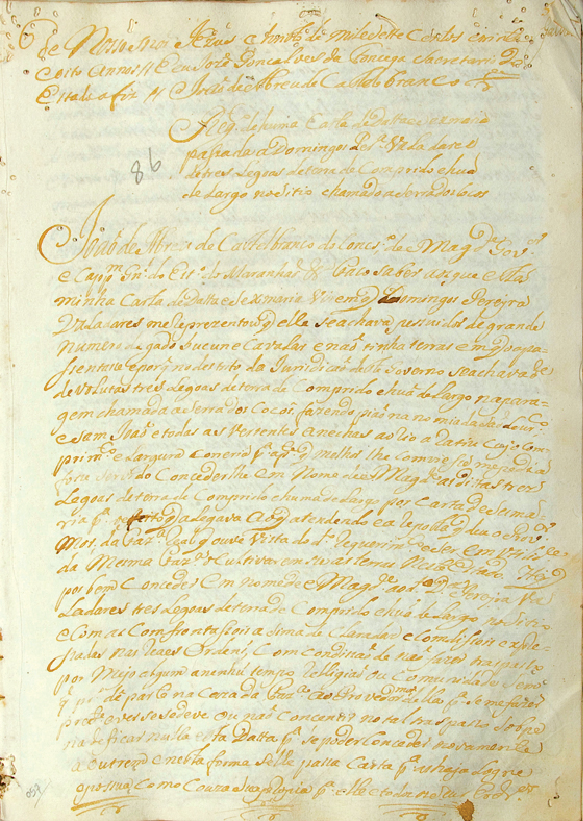
\includegraphics[width = \textwidth]
  {~/OneDrive - University of Illinois - Urbana/Research/Writing/git/Sesmarias/Pictures/0167f614a7c3b3fd38127f1545dbee7c.pdf}
  \end{subfigure}
  \begin{subfigure}[b]{0.6\textwidth}
  \centering
  %\vspace{-7.4cm}
  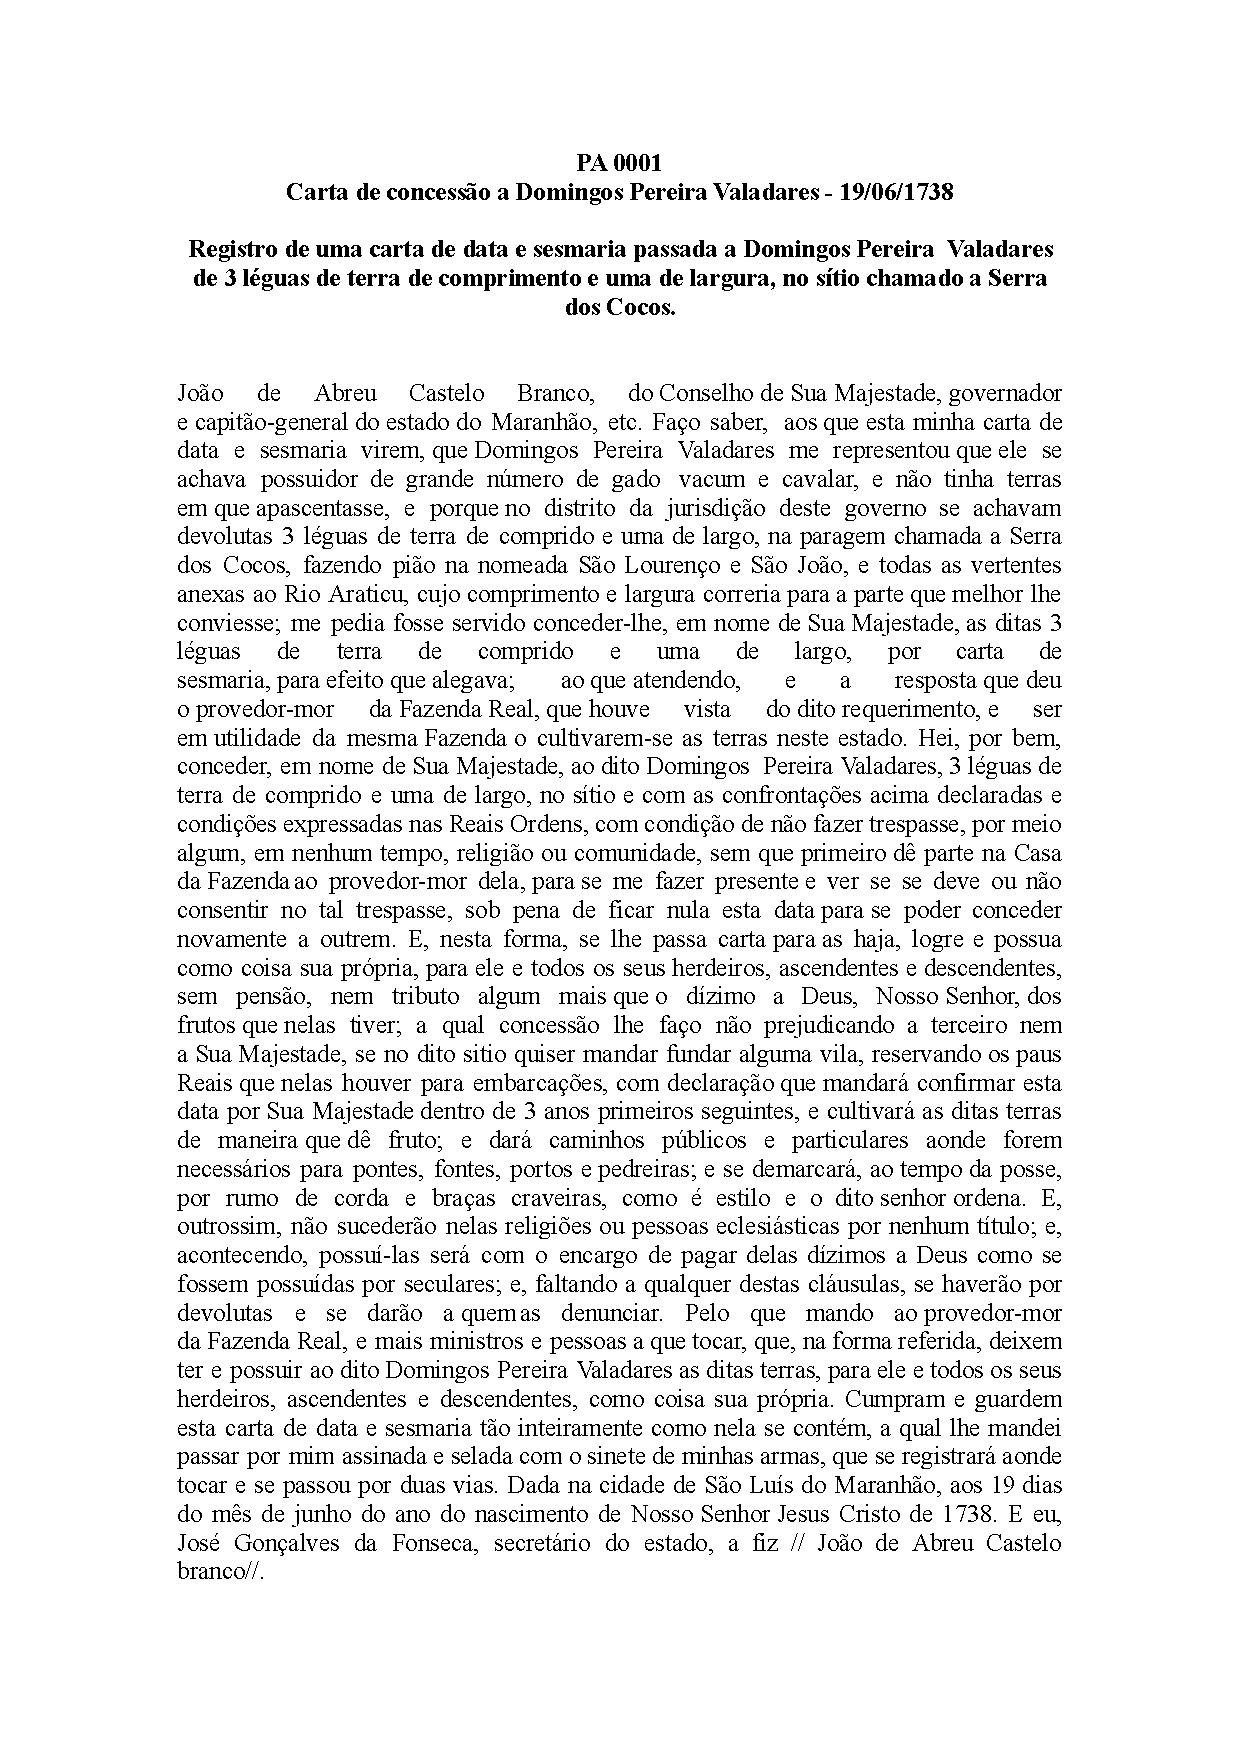
\includegraphics[page = 1, width = \textwidth]
  {~/OneDrive - University of Illinois - Urbana/Research/Writing/git/Sesmarias/Pictures/ea71ea6ac7c5ec3cefa24ded60ac6438.pdf}
  \end{subfigure}
  \end{center}
  \textit{Notes:} Example of an original manuscript and its transcribed version. Obtained from \textit{SILB} with the original source being from ...
\end{figure}
\end{landscape}

\clearpage

\begin{figure}[h!]
  \caption{Gridded Dataset for the Selected States}
  \begin{center}
     \makebox[\textwidth]			 
     {\includegraphics[width=\paperwidth]{/Users/vinicius/Library/CloudStorage/OneDrive-UniversityofIllinois-Urbana/Research/Projects/JMP/02. Figures/00.Maps/gridded_dataset.png}}
  \end{center}
  \textit{Notes:} Gridded dataset. Each square represents 0.1 x 0.1 degrees, which is approximately 10 x 10 km.  
  \label{fig:gridded_dataset}
\end{figure}

\clearpage

\begin{figure}[h!]
  \caption{Geographical distribution of Land Conflicts in Brazil}
  \begin{center}
     \makebox[\textwidth]			 
     {\includegraphics[width=0.75\paperwidth]{/Users/vinicius/Library/CloudStorage/OneDrive-UniversityofIllinois-Urbana/Research/Projects/JMP/02. Figures/00.Maps/cpt_conflict_data.png}}
  \end{center}
  \textit{Notes:} Geographical distribution of Land Conflicts in Brazil from 2014-2018 from [add source here]. Red dots indicate a conflict as reported on [add source here] alongside with 2010 municipality boundaries.
  \label{fig:cpt_conflict}
\end{figure}

\clearpage

\begin{figure}[h!]
  \caption{Land Grant Year Histogram}
  \begin{center}
     \makebox[\textwidth]			 
     {\includegraphics[width=0.75\paperwidth]{/Users/vinicius/Library/CloudStorage/OneDrive-UniversityofIllinois-Urbana/Research/Projects/JMP/02. Figures/00.Maps/slave_travels.png}}
  \end{center}
  \textit{Notes:} Histogram describing the yearly distribution of slave arrival ships from [add source here].  
  \label{fig:slave_distribution}
\end{figure}

\clearpage

\begin{figure}[h!]
  \caption{Land Grant Year Histogram}
  \begin{center}
     \makebox[\textwidth]			 
     {\includegraphics[width=0.75\paperwidth]{/Users/vinicius/Library/CloudStorage/OneDrive-UniversityofIllinois-Urbana/Research/Projects/JMP/02. Figures/00.Maps/slave_travels_region.png}}
  \end{center}
  \textit{Notes:} Histogram describing the yearly distribution of slave arrival ships from [add source here].  
  \label{fig:slave_distribution_region}
\end{figure}

\clearpage

\begin{figure}[h!]
  \caption{Distance to Explorer Route Histogram - 1872}
  \begin{center}
     \makebox[\textwidth]			 
     {\includegraphics[width=0.75\paperwidth]{/Users/vinicius/Library/CloudStorage/OneDrive-UniversityofIllinois-Urbana/Research/Projects/JMP/02. Figures/00.Maps/1872_IV_distance_hist.png}}
  \end{center}
  \textit{Notes:} Histogram describing the variation in the distance to the nearest explorer route for the 1872 parish level information.  
  \label{fig:1872_iv_hist}
\end{figure}


\clearpage

\begin{figure}[h!]
  \caption{1872 Municipalities and Parish Locations}
  \begin{center}
     \makebox[\textwidth]			 
     {\includegraphics[width=\paperwidth]{/Users/vinicius/Library/CloudStorage/OneDrive-UniversityofIllinois-Urbana/Research/Projects/JMP/02. Figures/00.Maps/parishes_1872.png}}
  \end{center}
  \textit{Notes:} Geographical distribution of 1872 parishes alongside 1872 municipality and state boundaries. The states to which I have information on the land grants are highlighted in red. This map shows that several municipalities, especially in the Southeastern states have more than one parish per municipality. The sample increases by using parish-level information instead of municipalities from 337 to 815.
  \label{fig:parishes_1872}
\end{figure}

\clearpage

[add here the image with the 1872 municipalities split alongside the parishes]

\clearpage

\begin{figure}[h!]
  \caption{\textit{Bandeira} Routes and 2010 Municipalities}
  \begin{center}
     \makebox[\textwidth]			 
     {\includegraphics[width=\paperwidth]{/Users/vinicius/Library/CloudStorage/OneDrive-UniversityofIllinois-Urbana/Research/Projects/JMP/02. Figures/00.Maps/bandeiras_dist_SE.png}}
  \end{center}
  \textit{Notes:} Proximity to a \textit{Bandeira} route and 2010 municipalities boundaries in the states of Sao Paulo and Minas Gerais. Red dots indicates the grants in those two states.
  \label{fig:bandeira_dist}
\end{figure}

\begin{figure}[h!]
  \caption{\textit{Bandeira} Routes and 2010 Municipalities \label{fig:bandeira_dist_graph}}
  \begin{center}
     \makebox[\textwidth]			 
     {\includegraphics[width=\paperwidth]{/Users/vinicius/Library/CloudStorage/OneDrive-UniversityofIllinois-Urbana/Research/Projects/JMP/02. Figures/00.Maps/1995_IV_distance_first_stage.png}}
  \end{center}
  \textit{Notes:} Proximity to a \textit{Bandeira} route and 2010 municipalities boundaries in the states of Sao Paulo and Minas Gerais. Red dots indicates the grants in those two states.
  \label{fig:bandeira_dist_graph}
\end{figure}

\begin{figure}[h!]
  \caption{\textit{Bandeira} Intersection and 2010 Municipalities}
  \begin{center}
     \makebox[\textwidth]			 
     {\includegraphics[width=\paperwidth]{/Users/vinicius/Library/CloudStorage/OneDrive-UniversityofIllinois-Urbana/Research/Projects/JMP/02. Figures/00.Maps/bandeiras_treat_SE.png}}
  \end{center}
  \textit{Notes:} Proximity to a \textit{Bandeira} route and 2010 municipalities boundaries in the states of Sao Paulo and Minas Gerais. Red dots indicates the grants in those two states.
  \label{fig:bandeiras_SE_treat}
\end{figure}

\begin{figure}[h!]
  \caption{Estimated Coefficients Excluding Municipalities Whose \% of Agricultural Units are above a cutoff}
  \begin{center}
     \makebox[\textwidth]			 
     {\includegraphics[width=0.8\paperwidth]{/Users/vinicius/Library/CloudStorage/OneDrive-UniversityofIllinois-Urbana/Research/Projects/JMP/02. Figures/00.Maps/robustness_cutoffs.png}}
  \end{center}
  \textit{Notes:} Red line indicates the main estimate based on.
  \label{fig:robustness_cutoffs}
\end{figure}

\clearpage

\section{Tables}

\input{~/OneDrive - University of Illinois - Urbana/Research/Projects/JMP/03. Tables/1995_Ag_Census_Land_Size_Varying.tex}

\clearpage

\section{Matching Descriptives}
\label{app:matching_checks}

\begin{landscape}
  \begin{figure}[htbp]
    \begin{center}
    \caption{Example original letter alongside its transcribed version}
    \label{fig:matching_1995}

    \begin{subfigure}[b]{0.3\linewidth}
    \centering
    \includegraphics[scale = 0.5]
    {~/OneDrive - University of Illinois - Urbana/Research/Projects/JMP/02. Figures/00.Maps/Matching_1995_All.png}
    \end{subfigure}

    \hfill

    \begin{subfigure}[b]{0.3\linewidth}
    \centering
    %\vspace{-7.4cm}
    \includegraphics[scale = 0.5]
    {~/OneDrive - University of Illinois - Urbana/Research/Projects/JMP/02. Figures/00.Maps/Matching_1995_1600.png}
    \end{subfigure}

    \hfill

    \begin{subfigure}[b]{0.3\linewidth}
    \centering
    %\vspace{-7.4cm}
    \includegraphics[scale = 0.5]
    {~/OneDrive - University of Illinois - Urbana/Research/Projects/JMP/02. Figures/00.Maps/Matching_1995_1700.png}
    \end{subfigure}

    \end{center}
    \textit{Notes:} Example of an original manuscript and its transcribed version. Obtained from \textit{SILB} with the original source being from ...
  \end{figure}
\end{landscape}

\begin{landscape}
  \begin{figure}[htbp]
    \begin{center}
    \caption{Example original letter alongside its transcribed version}

    \begin{subfigure}[b]{0.75\textwidth}
      \centering
      %\vspace{-7.4cm}
      \includegraphics[scale = 0.75]
      {~/OneDrive - University of Illinois - Urbana/Research/Projects/JMP/02. Figures/00.Maps/Matching_1995_1600.png}
    \end{subfigure}

    \begin{subfigure}[b]{0.75\textwidth}
      \centering
      %\vspace{-7.4cm}
      \includegraphics[scale = 0.75]
      {~/OneDrive - University of Illinois - Urbana/Research/Projects/JMP/02. Figures/00.Maps/Matching_1995_1700.png}
    \end{subfigure}

    \end{center}
    \textit{Notes:} Propensity Score Matching municipality selection for the 1995 Agricultural census. Blue municipalities represent municipalities that had at least one land grant within its boundaries, red represents the control municipalities. 
  \end{figure}
  \end{landscape}


\clearpage


\section{Data Source Appendix}
\label{app:data_source_appendix}

Below I describe the sources to which the land grants were compiled from. The states with a $^*$ indicate that the works was done by the researchers at SILB.

\vspace{2mm}

\textbf{Pernambuco$^*$}
\begin{itemize}
\item Documentação Histórica Pernambucana. Recife: Imprensa Oficial, 1954. Vol. 1-2
\item Documentação Histórica Pernambucana: sesmarias. Recife: Secretaria de Educação e Cultura. Biblioteca Pública, 1959. Vol. 1-4
\item Coleção Documentos Históricos Biblioteca Nacional do Rio de Janeiro. Vol. 20-22
\item Arquivo Nacional do Rio de Janeiro. Códice 427
\item Arquivo Nacional do Rio de Janeiro. Códice 155
\item Livro do Tombo do Mosteiro de São Bento de Olinda, Imprensa Oficial - Recife, 1948
\item Livros do Tombo de São Bento. Book 1-3
\item Revista do Instituto Arqueológico, Histórico e Geográfico Pernambucano, 1896.
\item Revista do Instituto Histórico de Goiana, 1871.
\end{itemize}

\textbf{Rio Grande do Norte$^*$}
\begin{itemize}
  \item O Treslado do auto e mais diligências que se fizeram sobre as datas de terras da capitania do Rio Grande, que se tinham dado. Fortaleza: Revista do Instituto do Ceará, 1909, Ano XXIII.
  \item IHGRN - Fundo Sesmarias - Books 1-9
  \item Documentos Históricos da Biblioteca Nacional do Rio de Janeiro..Vol. 23
  \item Documentos Históricos da Biblioteca Nacional do Rio de Janeiro..Vol. 24 Arquivo Nacional Rio de Janeiro, Códice 427
\end{itemize}

\textbf{Bahia$^*$}
\begin{itemize}
  \item Códice 427 - Rio de Janeiro
  \item FREIRE, Felisbello. História territorial do Brasil. Salvador: Secretaria da Cultura e Turismo, Instituto Geográfico e Histórico da Bahia, 1998
  \item DHBN - cartas publicadas na coleção Documentos Históricos da Biblioteca Nacional - DHBN, volumes 13 a 22
  \item  Anais do Arquivo Público do Estado da Bahia - Publicação dos anais do APEB - Anais do Arquivo Público do Estado da Bahia. Volumes 3 e 11
  \item Códice 155 - Rio de Janeiro
  \item Mosteiro de São Bento - Cartas publicadas nos Livros do Tombo do Mosteiro de São Bento  
\end{itemize}

\textbf{Paraiba$^*$}
\begin{itemize}
  \item British Library: Livro 1 (Land Grants (sesmarias) / Land Registers, 1757 - 1764); Livro 2: (Plots of Land 1722-1727 / Land Grants (sesmarias) 1722-1727); Livro 3: (Land Grants (sesmarias), 1785 -1787); Livro 4: (Land Grants (sesmarias), 1728 -1738); Livro 5: (Land Grants (sesmarias), 1816 - 1824); Livro 6: (Land Grants (sesmarias), 1747 - 1755); Livro 7: (Land Grants (sesmarias), 1789 - 1808); Livro 8: (Plots of Land - 1714-1717 / Land grants (sesmarias); Livro 9: (Land Grant - Various Parishes, 1768 - 1776); Livro 10: (Land Grants 1704-1722 / Sesmarias 1704-1722)
  \item TAVARES, João de Lira. Apontamentos para a História territorial da Parahyba. ed. Facsimilar. Brasília: Senado Federal, 1982. vol. CCXLV.
  \item Documentação Histórica Pernambucana: sesmarias. Recife:
  \item SECRETARIA DE EDUCAÇÃO E CULTURA BIBLIOTECA PÚBLICA, 1959
  \item Documentos Históricos da Biblioteca Nacional (DHBN): DHBN, V. 23. P.402-405.
  \item Códice 427 - Arquivo Nacional - Rio de Janeiro
  PUBLICAÇÕES DO ARCHIVO NACIONAL. VOL XXVII RIO DE
  JANEIRO Officinas Graphicas do ARCHIVO NACIONAL 1931. (Códice 155)
  \item Biblioteca Pública do Estado de Pernambuco (BPE) - Recife
  
\end{itemize}


\textbf{Sao Paulo}
\begin{itemize}
\item \textcite{noauthor_1921-qd} Vols. 1-3 
\item \textcite{Instituto-Historico-e-Geografico-de-Sao-Paulo1928-ej}
\end{itemize}

\textbf{Minas Gerais}
\begin{itemize}
  \item Revista do Arquivo Publico Mineiro - Inventory of the sesmarias letters on the Public Archive Codex - Volume 37 (1988)
  \item Revista do Arquivo Publico Mineiro - Volumes 10-24 (1905-1933). 
\end{itemize}

\clearpage

\section{Description of Letters and Georeferencing}
\label{app:appendix_data}

Below is a description on how the process used to georeference the land grants.

\begin{enumerate}
  \item Based on the letter information, since a location was required in order for the land to be granted, the geographical information on where the land was requested and who it was their neighbors is extracted.
  \item For example, the sesmaria of 
  \item It is also possible to georeference based on who the neighbors of the person were. 
  \begin{enumerate}
    \item For example, the sesmaria of Matheus Ferndandes Ramos which was granted in 1698, is described as being close to the sesmaria of Lucas Pedroso which was granted in 1638. 
  \end{enumerate}
  \item When not possible to georeference based on the above, the location is approximated at the municipality level. 
  \begin{enumerate}
    \item For example, in Minas Gerais, [...]
  \end{enumerate}
\end{enumerate}

Additionally, here are three practical examples on how each was georeferenced: 

\clearpage

\section{Parish Level Georeferencing}
\label{app:georeferencing_parishes}

The 1872 census was conducted at the parish level. For the 1872 census, the seven states that had a total of X municipalities, I georeferenced the information at the parish level for that census increasing the total sample size to X.

Below is a description of how the georeferencing was done:

\begin{enumerate}
  \item If the municipalities only had one parish, then the parish location is the same as the municipality seat.
  \begin{enumerate}
    \item The municipality of Serpa in Amazonas has only one parish, ``Nossa Senhora do Rosário de Serpa", therefore it is georeferenced to the municipality seat of Serpa.
  \end{enumerate}
  \item If a municipality has more than one parish, first I checked based on the name whether or not the parish level can be traced to a present-day city.
  \begin{enumerate}
    \item The municipality of Vigia in Para has three parishes: ``Nossa Senhora de Nazaré da Vigia", ``Nossa Senhora do Rosário de Collares", and ``São Caetano de Odivellas". 
    \item All of these parishes can be traced down to present-day cities, ``Nossa Senhora de Nazaré da Vigia" is the present-day municipality of Vigia, ``Nossa Senhora do Rosário de Collares" is the present-day municipality of Collares, and ``São Caetano de Odivellas" is the present-day municipality of São Caetano de Odivellas
  \end{enumerate}
  \item If the parish cannot be traced down based on the name to a present-day municipality then I took a look at other sources.\footnote{https://cidades.ibge.gov.br/ includes information on historical names for municipalities, based on their history.}
    \begin{enumerate}
      \item For example, the parish of [...] in the state of RJ cannot be traced by name to a present-day municipality, however, the church of the same name remains in the same place.
      \item Other maps such as [add the historical minas one here] were also used to identify old names of places.
    \end{enumerate}
\end{enumerate}

\clearpage

%\section{Coastal RDD - Results}
%\label{app:coastal_rdd}
%Given the setting of the coastal ban I estimate the following set of equations:
%\begin{equation}
%  Y_{m,s} = \beta \cdot CoastDist_{m,s} + f(D_{m,s})+ \mu_s + X_{m,s} + \epsilon_{m,s}
%\end{equation}

%For the 1970-2010 census, given that I have information at the individual level I estimate:
%\begin{equation}
%  Y_{i,m,s} = \beta \cdot CoastDist_{m} + f(D_{m})+ \mu_s + X_{i,m,s} + \epsilon_{i,m,s}
%\end{equation}

\section{Data Appendix - 1872}
\label{app:variable_construction_1872}

Below are the definitions of the variables measured for the 1872 census and how they were constructed. Some of the variables are already defined in the census:

\subsection{Base Variables, available by gender and free vs. enslaved:}

\begin{enumerate}
  \item Number of Literate People
  \item Number of People 6-15 Attending/Not Attending/No Information on Schooling
  \item Demographic Information on Race
    \begin{enumerate}
      \item Number of Enslaved People
      \item Number of Pardos
      \item Number of Whites
      \item Number of Blacks
      \item Number of Caboclos
    \end{enumerate}
  \item Number of People not born in the state based on origin: Within Brazil or from another country.
  \item Number of people on types of jobs: Liberal/Manual/Agricultural/Industry/Other Jobs/No Jobs
    \begin{enumerate}
      \item Liberal: Religious men/women, judges, lawyers, notaries, attorneys, justice officials, medics, surgeons, pharmacists, midwives, teachers, public officials, and artists.
      \item Manual or Mechanical: 
      \item Agricultural: Farmers and livestock breeders.
      \item Industry: Manufacturers and merchants.
      \item Other: Military officers, mariners, fishermen, capitalists/owners, \textit{jornaleiros} (workers that are paid based on a working day), domestic workers, and no information
    \end{enumerate}
  \item Number of people by age group.
\end{enumerate}

\subsection{Constructed Variables:}

\begin{enumerate}
  \item Number of Free People Above the Age of 15
  $$ \sum \text{\# Of Free People Above 15} $$

  \item Literacy Rates, following \textcite{Rocha2017-yq}: 
  $$100 \times \frac{\text{\# of Literate Free People}}{\text{\# of Free People Above the Age of 15}}$$

  \item Men Literacy Rates: 
  $$100 \times \frac{\text{\# of Literate Free Men}}{\text{\# of Free Men Above the Age of 15}}$$

  \item Women Literacy Rates: 
  $$100 \times \frac{\text{\# of Literate Free Women}}{\text{\# of Free Women Above the Age of 15}} $$

  \item Total number of children between 6-15
  \begin{equation*}
    \begin{array}{l}
  \text{\# of Free People between the ages 6-15 who attend school} + \\ \text{\# of Free People between the ages 6-15 who do not attend school} + \\ \text{\# of Free People between the ages 6-15 with no information on schooling}
    \end{array}
  \end{equation*}

  \item Percentage of Children between age 6-15 who are attending school:
  \begin{equation*}
    100 \times \frac{\text{\# of Free People between the ages 6-15 who attend school}}{\text{Total \# of Free Children between 6-15}}
  \end{equation*}

  \item Percentage of Boys between age 6-15 who are attending school:
  \begin{equation*}
    100 \times \frac{\text{\# of Free Boys between the ages 6-15 who attend school}}{\text{Total \# of Free Boys between 6-15}}
  \end{equation*}

  \item Percentage of Girls between age 6-15 who are attending school:
  \begin{equation*}
    100 \times \frac{\text{\# of Free Girls between the ages 6-15 who attend school}}{\text{Total \# of Free Girls between 6-15}}
  \end{equation*}

  \item Proportion of Slaves to Free Population:
  $$ 100 \times \frac{\text{\# of Enslaved People}}{\text{\# of Free People}} $$

  \item Proportion of White/Caboclo/Black/Pardo:
  $$ 100 \times \frac{\text{\# of Free People of Certain Race}}{\text{\# of Free People}}$$

  \item Proportion of Internal/Foreign Immigrants:
  $$ 100 \times \frac{\text{\# of Free People of Certain Immigration Category}}{\text{\# of Free People}}$$
  \item Proportion of Teachers per 10,000:
  $$ 10000 \times \frac{\text{\# of Free People working as Teacher}}{\text{\# of Free People}}$$
  \item Proportion of Workers by Labor Market characteristics (as described in the data above):
  $$ 100 \times \frac{\text{\# of Total People in Certain Job}}{\text{\# of Total People}}$$
\end{enumerate}

\end{document}